





%
%
%    This file contains portions of ../paper/LLADD-Frenix.tex that have
%    not yet made it into the file LLADD.tex in this directory.  If a section
%    of this file belongs in the new paper, *cut* it from this file, and paste 
%    it into the new version.  (This makes it easier to keep track of material 
%    that we're intentionally cutting, and prevents us from incorporating the 
%    same material into the new version twice...
%
%














%% LyX 1.3 created this file.  For more info, see http://www.lyx.org/.
%% Do not edit unless you really know what you are doing.
%\documentclass[letterpaper,twocolumn,english]{article}
%\usepackage[T1]{fontenc}
%\usepackage[latin1]{inputenc}
%\usepackage{graphicx}

\documentclass[letterpaper,twocolumn,english]{article}
\usepackage[latin1]{inputenc}
\usepackage{graphicx}
\usepackage{usenix,epsfig}


%\makeatletter


%\documentclass{article}
%\usepackage{usenix,epsfig,twocolumn}


%%%%%%%%%%%%%%%%%%%%%%%%%%%%%% LyX specific LaTeX commands.
%% Bold symbol macro for standard LaTeX users
%\newcommand{\boldsymbol}[1]{\mbox{\boldmath $#1$}}


%%%%%%%%%%%%%%%%%%%%%%%%%%%%%% User specified LaTeX commands.
\usepackage[T1]{fontenc}
\usepackage{ae,aecompl}

%\usepackage{babel}
%\makeatother

\begin{document}

\date{}

\title{\Large \bf LLADD: An Extensible Transactional Storage Layer\\
  \normalsize{(yaahd)}}

\author{
Russell Sears  and  Eric Brewer\\
{\em UC Berkeley}\\
% is there a standard format for email/URLs??
% remember that ~ doesn't do what you expect, use \~{}.
{\normalsize \{sears,brewer\}@cs.berkeley.edu, http://lladd.sourceforge.net} \\
%
% copy the following lines to add more authors
% \smallskip
% Name Two Here \\
%{\em Two's Institution}\\
%% is there a standard format for email/URLs??
%{\normalsize two@host.site.dom, http://host.site.dom/twourl}
%
} % end author

\maketitle

\thispagestyle{plain}

\section{Introduction}

Changes in data models, consistency requirements, system scalability,
communication models and fault models require changes to the storage
and recovery subsystems of modern applications. 

% rcs:##1##
For applications that are willing to store all of their data in a
DBMS, and access it only via SQL, existing databases are just fine and
LLADD has little to offer.  However, for those applications that need
more direct management of data, LLADD offers a layered architecture
that enables simple but robust data management.\footnote{A large class
of such applications are deemed ``navigational'' in the database
vocabulary, as they directly navigate data structures rather than
perform set operations.}
We also believe that LLADD is applicable in
the context of new, special-purpose database systems such as XML databases,
streaming databases, and extensible/semantic file systems~\cite{reiser, semantic}.  These form a 
fruitful area of current research,~\cite{newTypes} but existing monolithic database systems tend to be a poor fit for these new areas.

The basic approach of LLADD, taken from ARIES~\cite{aries}, is to build
\emph{transactional pages}, which enables recovery on a page-by-page
basis, despite support for high concurrency and the minimization of
disk seeks during commit (by using a log).  We show how to build a variety
of useful data managers on top of this layer, including persistent
hash tables, lightweight recoverable virtual memory (LRVM)~\cite{lrvm}, and simple
databases.  We also cover the details of crash recovery,
application-level support for transaction abort and commit, and latching for multi-threaded applications.
Finally, we discuss the shortcomings of a few common applications, and explain
why LLADD provides an appropriate solution to these problems.

%[more coverage of kinds of apps?  imap, lrvm, cht, file system, database]

%rcs: is this paragraph old news?  cut everything but the last sentence?
Many implementations of transactional pages exist in industry and
in the literature. Unfortunately, these algorithms tend either to
be straightforward and unsuitable for real-world deployment, or are
robust and scalable, but achieve these properties by relying upon
intricate sets of internal and often implicit interactions. The
ARIES algorithm falls into the second category, and has been extremely
successful as part of the IBM DB2 database system.
It provides performance and reliability that is comparable to that of current
commercial and open-source products. Unfortunately, while the algorithm
is conceptually simple, many subtleties arise in its implementation.
We chose ARIES as the basis of LLADD, and have made a significant
effort to document these interactions. Although  a complete discussion
of the ARIES algorithm is beyond the scope of this paper, we will
provide a brief overview and explain the details that are relevant
to developers that wish to extend LLADD. 

By documenting the interface between ARIES and higher-level primitives
such as data structures and by structuring LLADD to make this
interface explicit in both the library and its extensions, we hope to
make it easy to produce correct and efficient durable data
structures. In existing systems (and indeed, in earlier versions of
LLADD), the implementation of such structures is extremely
complicated, and subject to the introduction of incredibly subtle
errors that would only be evident during crash recovery or at other
inconvenient times.  Thus there is great value in reusing lower layers.

Finally, by approaching this problem by implementing a number of simple
modules that ``do one thing and do it well'', we believe that
LLADD can provide competitive performance while making future improvements
to its core implementation significantly easier. In order to achieve
this goal, LLADD has been split into a number of modules forming a
{\em core library}, and a number of extensions called {\em operations} that
build upon the core library. Since each of these modules exports a
stable interface, they can be independently improved.


\subsection{Prior Work\label{sub:Prior-Work}}

An extensive amount of prior work covers the algorithms presented in
this paper.  Most fundamentally, systems that provide transactional
consistency to their users generally include a number of common
modules.  Figure~\ref{cap:DB-Architecture} presents a high-level overview of a typical system.

\begin{figure}
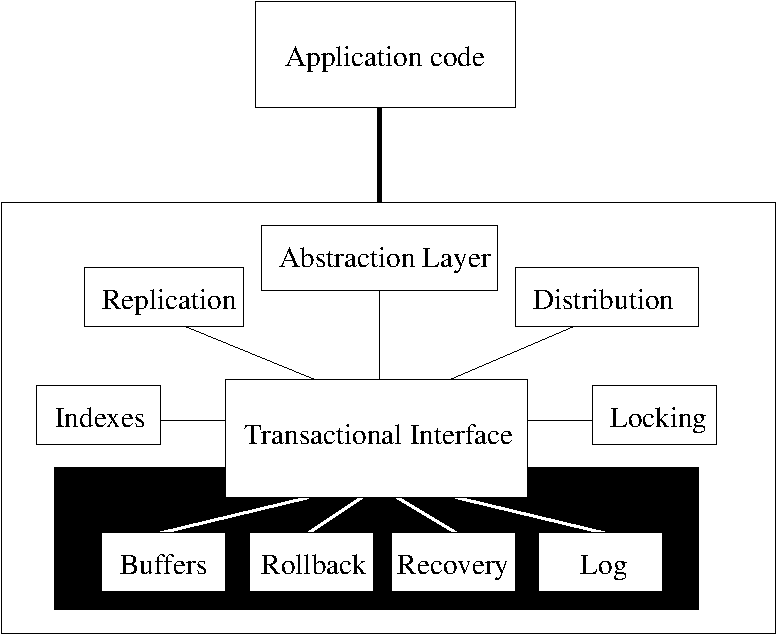
\includegraphics[%
  width=1.0\columnwidth]{DB-Architecture.pdf}


\caption{\label{cap:DB-Architecture}Conceptual view of a modern
transactional application.  Current systems include high-level
functionality, such as indices and locking, but are not designed to
allow developers to replace this functionality with
application-specific modules.}
\end{figure}

Many systems make use of transactional storage that is
designed for a specific application or set of applications.  LLADD
provides a flexible substrate that allows such systems to be
developed easily.  The complexity of existing systems varies widely, as do
the applications for which these systems are designed.  


We have only provided a small sampling of the many applications that
make use of transactional storage.  Unfortunately, it is extremely
difficult to implement a correct, efficient and scalable transactional
data store, and we know of no library that provides low-level access
to the primitives of such a durability algorithm.  These algorithms
have a reputation of being complex, with many intricate interactions,
which prevent them from being implemented in a modular, easily
understandable, and extensible way.  

Because of this, many applications that would benefit from
transactional storage, such as CVS and many implementations of IMAP,
either ignore the problem, leaving the burden of recovery to system
administrators or users, or implement ad-hoc solutions that employ
complex, application-specific storage protocols in order to ensure
the consistency of their data.  This increases the complexity of such
applications and often provides only a partial solution to the
transactional storage problem, resulting in erratic and unpredictable
application behavior.

In addition to describing a flexible implementation of ARIES, a well-tested
``industrial strength'' algorithm for transactional storage, this paper
outlines the most important interactions in ARIES (that
is, the ones that could not or should not be encapsulated within our
implementation), and gives the reader a sense of how to use the
primitives the library provides.


\section{LLADD Architecture}

%
\begin{figure}
~~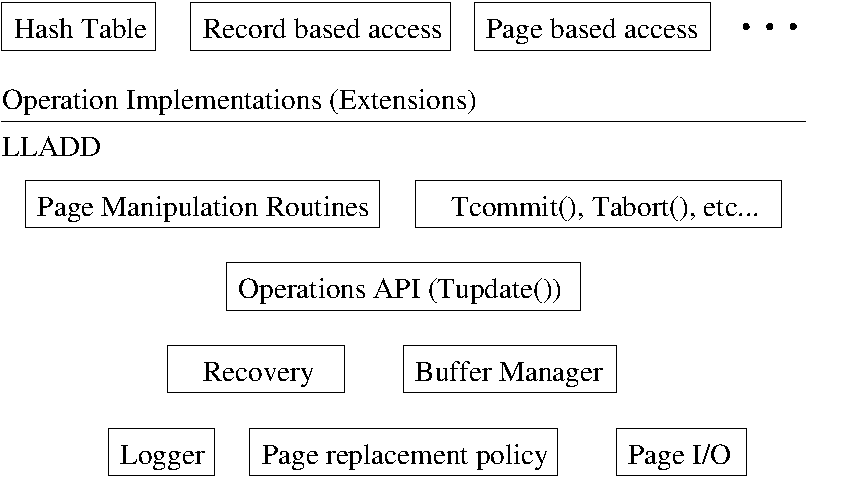
\includegraphics[%
  width=1.0\columnwidth]{LLADD-Arch3.pdf}

\caption{\label{cap:LLADD-Architecture}Simplified LLADD Architecture: The
core of the library places as few restrictions on the application's
data layout as possible. Custom {}``operations'' implement the client's
desired data layout. The separation of these two sets of modules makes
it easy to improve and customize LLADD.}
\end{figure}
LLADD is a toolkit for building transaction managers.
It provides user-defined redo and undo behavior, and has an extendible
logging system with 19 types of log entries so far (not counting those
internal to LLADD, such as ``begin'', ``abort'', and ``clr''). Most of these
extensions deal with data layout or modification, but some deal with
other aspects of LLADD, such as extensions to recovery semantics (Section
\ref{sub:Two-Phase-Commit}). LLADD comes with some default page layout
schemes, but allows its users to redefine this layout as is appropriate.
Currently LLADD imposes two requirements on page layouts. The first
32 bits must contain an LSN for recovery purposes,
and the second 32 bits must contain the page type (since we allow multiple page formats).

Although it ships with basic operations that support variable-length
records, hash tables and other common data types, our goal is to
decouple all decisions regarding data format from the implementation
of the logging and recovery systems. Therefore, the preceding section
is essentially documentation for users of the library, while
the purpose of the performance numbers in our evaluation section are
not to validate our hash table, but to show that the underlying architecture
is able to efficiently support interesting data structures.

Despite the complexity of the interactions among its modules, the
basic ARIES algorithm itself is quite simple. Therefore, in order to
keep LLADD simple, we started with a set of modules, and iteratively
refined the boundaries among these modules. Figure~\ref{cap:LLADD-Architecture} presents the resulting architecture.  The
core of the LLADD library is quite small at 2218 lines of code, 2155
lines of implementations of operations and other extensions, and 408
lines of installable header files.\footnote{These counts were generated using David
A. Wheeler's {\tt SLOCCount}.} The code has been documented extensively,
and we hope that we have exposed most of the subtle interactions
among internal modules in the online documentation.

As LLADD has evolved, many of its sub-systems have been incrementally
improved, and we believe that the current set of modules is amenable
to the addition of new functionality. For instance, the logging module
interface encapsulates all of the details regarding its on disk format,
which allows for some of the exotic logging and replication techniques mentioned above.
Similarly, the interface encodes the dependencies
between the logger and other subsystems.%
\footnote{For example, the buffer manager must ensure that the logger has forced the appropriate
log entries to disk before writing a dirty page to disk. Otherwise,
it would be impossible to undo the changes that had been made to the
page.%
}

The buffer manager is another potential area for extension.
Because the interface between the buffer manager and LLADD is simple,
we would like to support transactional access to resources beyond
simple page files. Some examples include transactional updates of
multiple files on disk, transactional groups of program executions
or network requests, or even leveraging some of the advances being
made in the Linux and other modern OS kernels. For example,
ReiserFS recently added support for atomic file-system operations.
This could be used to provide variable-sized pages
to LLADD.  We revisit these ideas when we discuss existing systems 
such as CVS and IMAP, although they are applicable in many other 
circumstances.

From the testing point of view, the advantage of LLADD's division
into subsystems with simple interfaces is obvious. We are able to
use standard unit-testing techniques to test each of LLADD's subsystems
independently, and have documented both external and internal interfaces,
making it easy to add new tests and debug old ones. Furthermore, by
adding a ``simulate crash'' operation to a few of the key components,
we can simulate application level crashes by clearing LLADD's internal
state, re-initializing the library and verifying that recovery was
successful. These tests currently cover approximately 
90\%\footnote{generated using ``gcov'', and ``lcov,''}
of the code. We have not yet developed a mechanism that models hardware failures, but plan to develop a test harness that verifies operation behavior in exceptional circumstances.

LLADD's performance requirements vary wildly depending on the workload
with which it is presented. Its performance on a large number of small,
sequential transactions will always be limited by the amount of time
required to flush a page to disk. To some extent, compact logical
and physiological log entries improve this situation. On the other
hand, long running transactions only rarely force-write to disk and
become CPU bound. Standard profiling techniques of the overall library's
performance and micro-benchmarks of crucial modules handle such situations
nicely. 

Each module of LLADD is reentrant, and a
C preprocessor directive allows the entire library to be instrumented
in order to profile latching behavior, which aids in performance
tuning and debugging. A thread that is not involved in
an I/O request never needs to wait for a latch held by a thread that
is waiting for I/O.%
\footnote{Strictly speaking, this statement is only true for LLADD's core.
However, there are variants of most popular data structures that allow
us to preserve these invariants.%
}

There are a number of performance optimizations that are specific
to multi-threaded operations that we do not perform. The most glaring
omission is log bundling; if multiple transactions commit at once,
LLADD must still force the log to disk once per transaction. This problem
is not fundamental, but simply has not been addressed by current code
base. Similarly, as page eviction requires a force-write if the
full ARIES recovery algorithm is in use, we could implement a thread
that asynchronously maintained a set of free buffer pages. We plan to 
implement such optimizations in the future.


\section{Sample Operations}

In order to validate LLADD's architecture, and to show that it simplifies
the creation of efficient data structures, we have have implemented
a number of simple extensions. In this section, we describe their
design, and provide some concrete examples of our experiences extending
LLADD.  We would like to emphasize that this discussion reflects a 
``worst case'' scenario; if LLADD extensions appropriate for an application 
already exist, the process detailed in this section is unnecessary.  If an 
application does not require concurrent, multi-threaded applications, then 
physical logging can be used, allowing for the extremely simple 
implementation of new operations.


The bucket list must be addressable as though it was an expandable array. We have implemented
this functionality as a separate module reusable by applications, but will not discuss it here.

For the purposes of comparison, we provide two linear hash implementations.
The first is straightforward, and is layered on top of LLADD's standard
record setting operation, Tset(), and therefore performs physical
undo. This implementation provided a stepping stone to the more sophisticated
version which employs logical undo, and uses an identical on-disk
layout. As we discussed earlier, logical undo provides more opportunities
for concurrency, while decreasing the size of log entries. In fact,
the physical-undo implementation of the linear hash table cannot support
concurrent transactions, while threads utilizing the logical-undo 
implementation never hold locks on more than two buckets.%
\footnote{However, only one thread may expand the hash-table at once.  In order to amortize the overhead of initiating an expansion, and to allow concurrent insertions, the hash table is expanded in increments of a few thousand buckets.}
We see some performance improvement due to logical logging in Section~\ref{sec:eval}.

\begin{figure}
\begin{center}
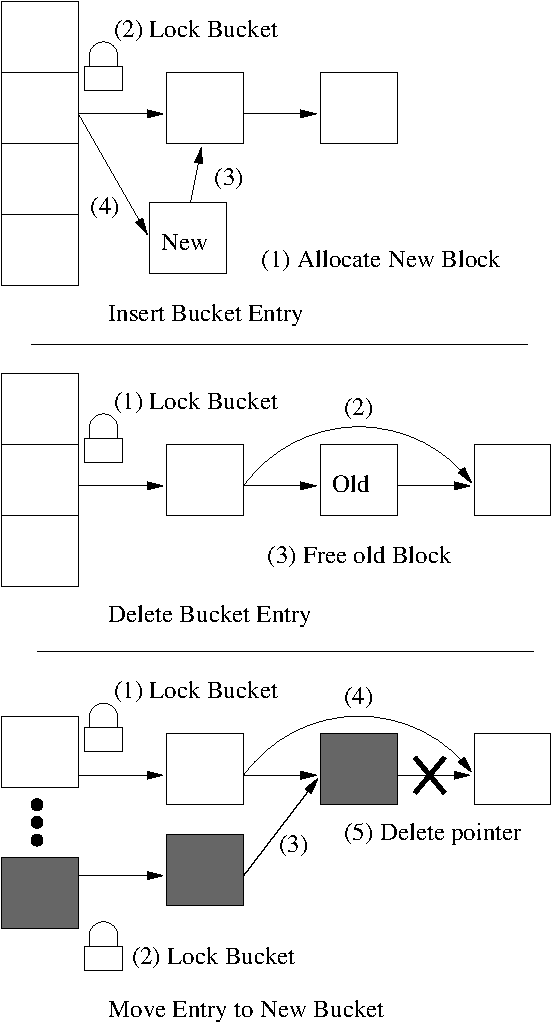
\includegraphics[%
  width=0.70\columnwidth]{LinkedList.pdf}
\end{center}

\caption{\label{cap:Linear-Hash-Table}Linear Hash Table Bucket operations.}
\end{figure}


From our point of view, the linked list management portion of the hash 
table algorithm is particularly interesting.  It is straightforward in the
physical case, but must be performed in a specific order in the logical
case. See Figure \ref{cap:Linear-Hash-Table} for a sequence of steps
that safely implement the necessary linked list operations. Note that
in the first two cases, the portion of the linked list that is visible
from LLADD's point of view is always logically consistent. This is important
for crash recovery; it is possible that LLADD will crash before the
entire sequence of operations has been completed. The logging protocol
guarantees that some prefix of the log will be available. Therefore,
because the run-time version of the hash table is always consistent,
we know that the version of the hash table produced by the REDO phase 
of recovery will also be consistent.  Note that we have to worry about ordering because the buffer
manager only provides atomic updates of single pages, but our linked list may span pages.

The third case, where buckets are split as the bucket list is expanded,
is a bit more complicated. We must maintain consistency between two
linked lists, and a page at the beginning of the hash table that contains
the last bucket that we successfully split. Here, we use the undo
entry to ensure proper crash recovery, not by undoing the split, but 
by actually redoing it; this is a perfectly valid ``undo'' strategy for some operations.
Our bucket split algorithm
is idempotent, so it may be applied an arbitrary number of times to
a given bucket with no ill-effects. Also note that in this case
there is not a good reason to undo a bucket split, so we can safely
apply the split whether or not the current transaction commits.

First, we write an ``undo'' record that checks the hash table's meta-data and
redoes the split if necessary (this record has no effect 
unless we crash during this bucket split). Second, we write (and execute) a series
of redo-only records to the log. These encode the bucket split, and follow
the linked list protocols listed above. Finally, we write a redo-only
entry that updates the hash table's meta-data.%
\footnote{Had we been using nested top actions, we would not need the special
undo entry, but we would need to store {\em physical} undo information for
each of the modifications made to the bucket, since any subset of the pages may have been stolen.%
}

We allow pointer aliasing at this step so that a given key can be
present for a short period of time in both buckets. If we crash before
the undo entry is written, no harm is done. If we crash after the
entire update makes it to log, the redo stage will set the hash's
meta-data appropriately, and the undo record becomes a no-op. If
we crash in the middle of the bucket split, we know that the current
transaction did not commit, and that recovery will execute the undo
record. It will see that the bucket split is still pending and finish
splitting the bucket. Therefore, the hash table is correctly restored. 

Note that there is a point during the undo phase where the bucket
is in an inconsistent physical state.  Normally the redo phase
brings the page file to a fully consistent physical state.
We handle this by obtaining a lock on the bucket during normal
operation. This blocks any attempt to write log entries
that alter a bucket while it is being split.  Therefore, the log 
cannot contain any entries that will accidentally attempt to
access an inconsistent bucket.

Since the second implementation of the linear hash table uses logical
undo, we are able to allow concurrent updates to different portions
of the table. This is not true in the case of the implementation that
uses pure physical logging, as physical undo cannot generally tolerate
concurrent structural modifications to data structures.


\subsection{Two-Phase Commit\label{sub:Two-Phase-Commit}}

The two-phase commit protocol is used in clustering applications where
multiple, well maintained, well connected computers must agree upon
a set of successful transactions. Some of the systems could crash,
or the network could fail during operation, but we assume that such
failures are temporary. Two-phase commit designates a single computer
as the coordinator of a given transaction. This computer contacts
the other systems participating in the transaction, and asks them
to prepare to commit. If a subordinate system sees
that an error has occurred, or the transaction should be aborted for
some other reason, then it informs the coordinator. Otherwise, it
enters the \emph{prepared} state, and tells the coordinator that it
is ready to commit. At some point in the future the coordinator will
reply, telling the subordinate to commit or abort. From LLADD's point
of view, the interesting portion of this algorithm is the \emph{prepared}
state, since it must be able to commit a prepared transaction if it
crashes before the coordinator responds, but cannot commit before
hearing the response, since it may be asked to abort the transaction.

Implementing the prepare state on top of the ARIES algorithm consists
of writing a special log entry that informs the undo portion of the
recovery phase that it should stop rolling back the current transaction
and instead add it to the list of active transactions.%
\footnote{Also, any locks that the transaction obtained should be restored,
which is outside of the scope of LLADD, although a LLADD operation could 
easily implement this functionality on behalf of an external lock manager.%
} Due to LLADD's extendible logging system, and the simplicity
of its recovery code, it took an afternoon for a programmer to become familiar with LLADD's
architecture and add the prepare operation.  This implementation of prepare allows
LLADD to support applications that require two-phase commit.  A preliminary 
implementation of a cluster hash table that employs two-phase
commit is included in LLADD's CVS repository.

\subsection{Other Applications}

Previously, we mentioned a few systems that we think would benefit
from LLADD.  Here we sketch the process of implementing such
applications.  

LRVM implements a transactional version of malloc() \cite{lrvm}.  It
employs the operating system's virtual memory system to generate page
faults if the application accesses a portion of memory that has not
been swapped in.  These page faults are intercepted and processed by a
transactional storage layer which loads the corresponding pages from
disk.  A few simple functions such as abort() and commit() are
provided to the application, and allow it to control the duration of
its transactions.  LLADD provides such a layer and the necessary
calls, reducing the LRVM implementation to an implementation of the
page fault handling code.  The performance of the transactional
storage system is crucial for this sort of application, and the
variable length, keyed access, and higher levels of abstraction
provided by existing libraries impose a severe performance penalty.  LLADD could easily
be extended so that it employs an appropriate on-disk structure that
provides efficient, offset based access to aligned, fixed length
blocks of data.  A, LRVM requires a set\_range() operation
that efficiently updates a portion of a record, saving logging overhead.
This feature could also be implemented as an operation, providing a simple,
fast version of LRVM that would benefit from the infrastructure
surrounding LLADD.

CVS provides version control over large sets of files.  Multiple users
may concurrently update the repository of files, and CVS attempts to
merge conflicts and maintain the consistency of the file tree.  By
adding the ability to perform file system manipulations to LLADD, we
could easily support applications with requirements similar to those
of CVS.  Furthermore, we could combine the file-system manipulation
with record-oriented storage to store application-level logs, and
other important meta-data.  This would allow a single mechanism to
support applications such as CVS, simplifying fault tolerance, and
improving the scalability of such applications.

IMAP is similar to CVS, but benefits further since it uses a simple,
folder-based locking protocol, which would be extremely easy to
implement using LLADD.

These last two examples highlight some of the potential advantages of
extending LLADD to manipulate the file system, although it is possible
that LLADD's page file would provide improved performance over the
file system, at the expense of the transparency
of file-system based storage mechanisms.

%[cite j2ee in next paragraph]

Another area of interest is in transactional serialization mechanisms
for programming languages.  Existing solutions are often complex, or
are layered on top of a relational database or other system that uses
a data format that is different than the representation the
programming language uses.  J2EE implementations and the wide variety of 
other persistence mechanisms
available for Java provide a nice survey of the potential design
choices and tradeoffs.  Since LLADD can easily be adapted to an
application's desired data format, we believe that it is a good match
for such persistence mechanisms.

\section{\label{sec:eval} Performance}

We hope that the preceding sections have given the reader an idea
of the usefulness and extensibility of the LLADD library. In this
section we focus on performance evaluation.

In order to evaluate the physical and logical hash-table implementations,
we first ran a test that inserts some tuples into the database. For
this test, we chose fixed-length (key, value) pairs of integers. For
simplicity, our hash-table implementations currently only support fixed-length
keys and values, so this this test puts us at a significant advantage.
It also provides an example of the type of workload that LLADD handles
well; LLADD is designed to support application
specific transactional data structures.  For comparison, we also ran 
``Record Number'' trials, named after the Berkeley DB access method.  
In this case, data is essentially stored in a large on-disk array.  This test provides a measurement of the speed of the 
lowest level primitive supported by Berkeley DB, and the corresponding LLADD extension. 

%
\begin{figure*}
\begin{center}
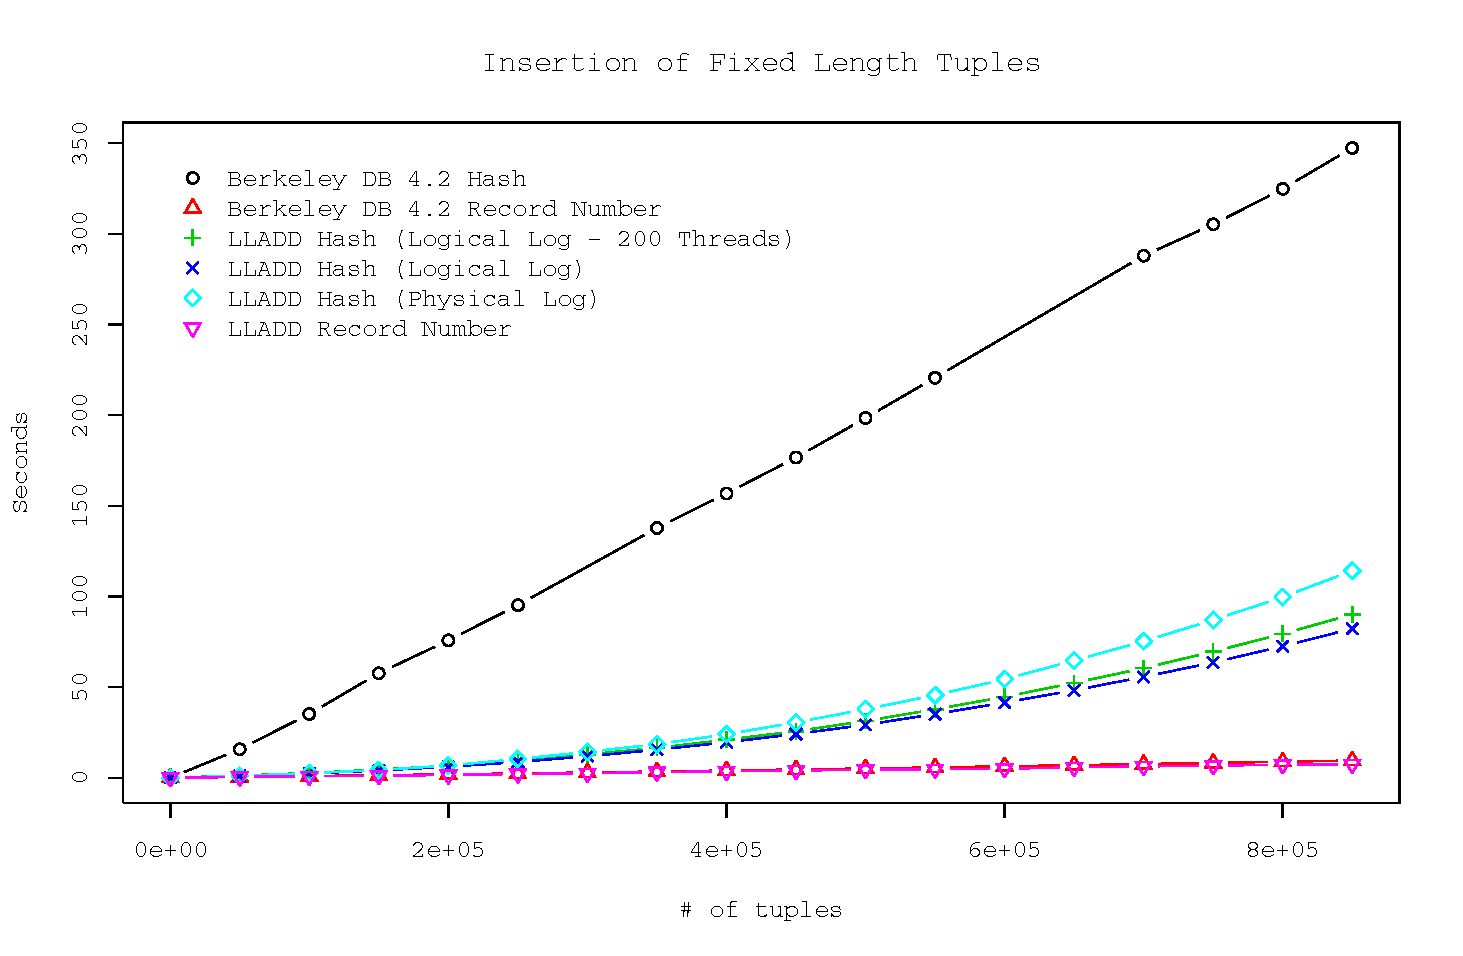
\includegraphics[%
  width=0.75\textwidth]{INSERT.pdf}
\end{center}

\caption{\label{cap:INSERTS}The final data points for LLADD's and Berkeley
DB's record number based storage are 7.4 and 9.5 seconds, respectively.
LLADD's hash table is significantly faster than Berkeley DB in this
test, but provides less functionality than the Berkeley DB hash. Finally,
the logical logging version of LLADD's hash table is faster than the
physical version, and handles the multi-threaded test well. The threaded
test spawned 200 threads and split its workload into 200 separate transactions.}
\end{figure*}

%
\begin{figure*}
\begin{center}
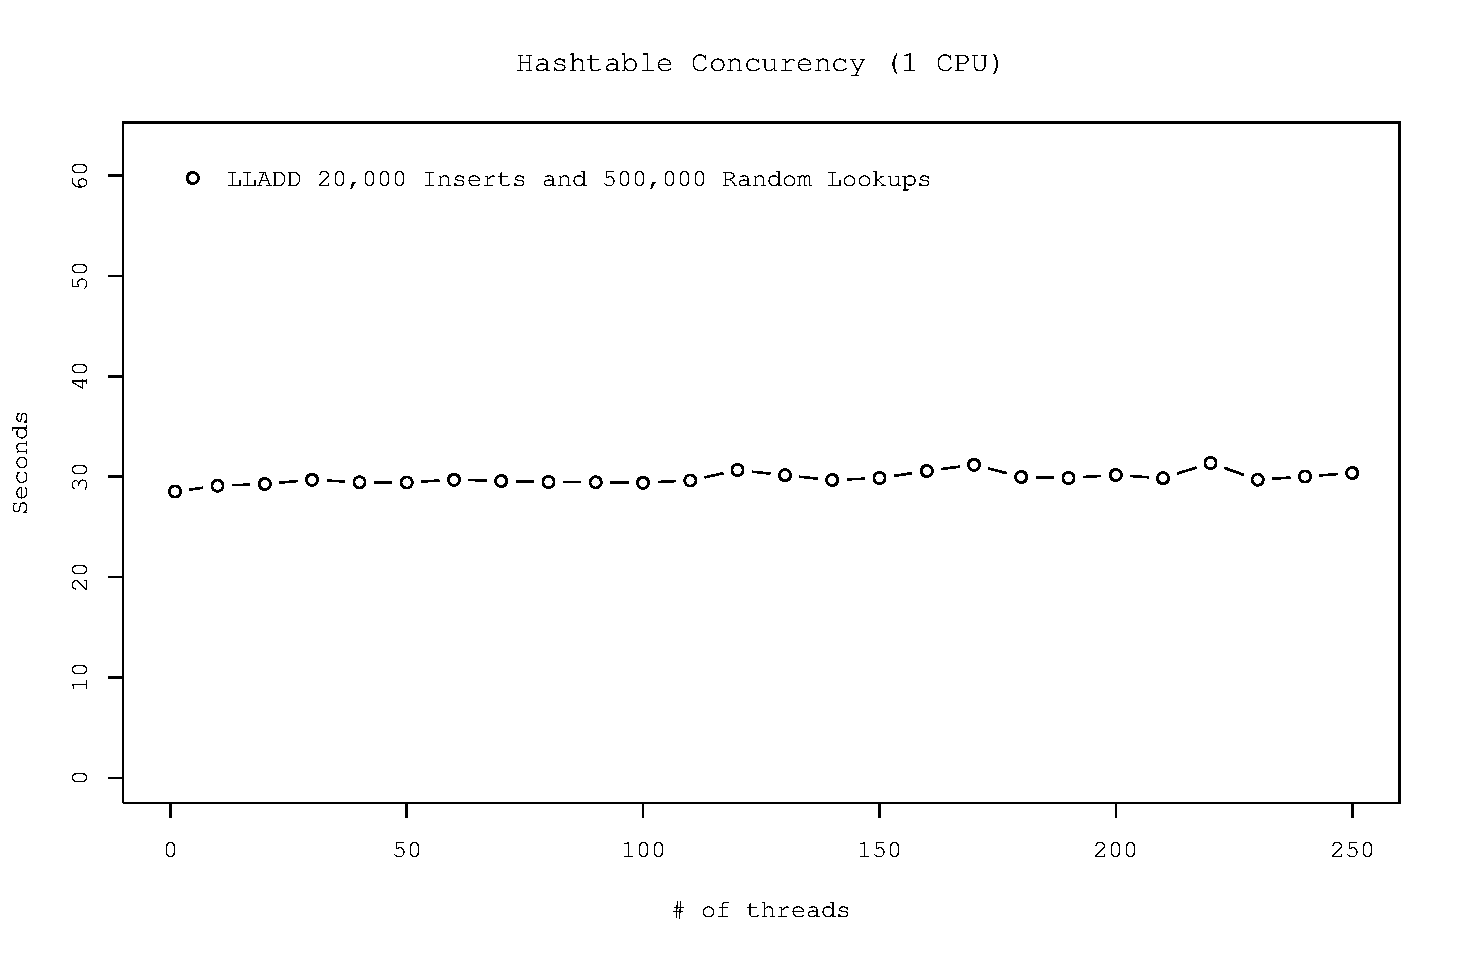
\includegraphics[%
  width=0.75\textwidth]{THREADS-sparse.pdf}
\end{center}
\caption{\label{cap:THREADS}The time required to perform a fixed
amount of processing, split across various numbers of threads.  This
test was run against the highly concurrent Logical Logging version of
the linear hash table.  No significant performance degradation was
seen within the range measured.  The inserts were done in serial, and
the lookups were performed in parallel.}
\end{figure*}


The times included in Figure \ref{cap:INSERTS} include page file
and log creation, insertion of the tuples as a single transaction,
and a clean program shutdown. We used the ``transapp.cs'' program from
the Berkeley DB 4.2 tutorial to run the Berkeley DB tests, and hard-coded
it to use integers instead of strings. We used the Berkeley DB {}``DB\_HASH''
index type for the hash-table implementation, and {}``DB\_RECNO''
in order to run the {}``Record Number'' test.  

Since LLADD addresses records as \{Page, Slot, Size\} triples, which
is a lower level interface than Berkeley DB exports, we used the expandable
array that supports the hash-table implementation to run the {}``LLADD
Record Number'' test.

One should not look at Figure \ref{cap:INSERTS}, and conclude {}``LLADD
is almost five times faster than Berkeley DB,'' since we chose a
hash table implementation that is tuned for fixed-length data. Instead,
the conclusions we draw from this test are that, first, LLADD's primitive
operations are on par, performance wise, with Berkeley DB's, which
we find very encouraging. Second, even a highly tuned implementation
of a ``simple'' general-purpose data structure is not without overhead,
and for applications where performance is important a special purpose
structure may be appropriate.

%Also, the multi-threaded test run shows that the library is capable of
%handling a large number of threads. The performance degradation
%associated with running 200 concurrent threads was negligible.  Figure
%TODO expands upon this point by plotting the time taken for various
%numbers of threads to perform a total of 500,000 (TODO-CHECK) read operations.  The
%logical logging version of LLADD's hashtable outperformed the physical
The logical logging version of LLADD's hash-table outperformed the physical
logging version for two reasons.  First, since it writes fewer undo
records, it generates a smaller log file.  Second, in order to
emphasize the performance benefits of our extension mechanism, we use
lower level primitives for the logical logging version.  The logical
logging version implements locking at the bucket level, so many
mutexes that are acquired by LLADD's default mechanisms are redundant.
The physical logging version of the hash-table serves as a rough proxy
for an implementation on top of a non-extendible system.  Therefore,
it uses LLADD's default mechanisms, which include the redundant
acquisition of locks.

As a final note on our first performance graph, we would like to address
the fact that LLADD's hash-table curve is non-linear. LLADD currently
uses a fixed-size in-memory hash-table implementation in many areas,
and it is possible that we exceeded the fixed-size of this hash-table
on the larger test sets. Also, LLADD's buffer manager is currently
fixed size. Regardless of the cause of this non-linearity, we do not
believe that it is fundamental to our design.

The multi-threaded test run in the first figure shows that the library
is capable of handling a large number of threads. The performance
degradation associated with running 200 concurrent threads was
negligible.  Figure~\ref{cap:THREADS} expands upon this point by plotting the time
taken for various numbers of threads to perform a total of 500,000
 read operations.  The performance of LLADD in this figure
is essentially flat, showing only a negligible slowdown up to 250
threads.  (Our test system prevented us from spawning more than 250
simultaneous threads, and we suspect that LLADD would easily scale to more than 250 threads.  This test was
performed on a uniprocessor machine, so we did not expect to see a
significant speedup when we moved from a single thread to multiple
threads. 

Unfortunately, when ran this test on a multi-processor machine, we saw
a degradation in performance instead of the expected speed up.
The problem seems to be the additional overhead incurred by
multi-threaded applications running on SMP machines under Linux 2.6,
as the single thread test spent a small amount of time in the Linux
kernel, while even the two-thread version of the test spent a
significant time in kernel code.  We suspect that the large number of
briefly-held latches that LLADD acquires caused this problem.  We plan
to investigate this problem further, adopting LLADD to a more advanced
threading package with user-level latches~\cite{capriccio}, or providing an ``SMP Mode''  compile-time option that
decreases the number of latches that LLADD acquires at the expense of
opportunities for concurrency.

\section{Future Work}

LLADD is an extendible implementation of the ARIES algorithm. This
allows application developers to incorporate transactional recovery
into a wide range of systems. We have a few ideas along these lines,
and also have some ideas for extensions to LLADD itself.

LLADD currently relies upon its buffer manager for page-oriented storage.
Although we did not have space to discuss it in this paper, we have
a blob implementation that stores large data outside of the page file.
This concept could be extended to arbitrary primitives, such as transactional
updates to file system directory trees, or integration of networking
or other operations directly into LLADD transactions. Doing this would
allow LLADD to act as a sort of ``glue code'' among various systems,
ensuring data integrity and adding database-style functionality, such
as continuous backup, to systems that currently do not provide such
mechanisms. We believe that there is quite a bit of room for the development
of new software systems in the space between the high-level but sometimes
inappropriate interfaces exported by existing transactional storage systems, 
and the unsafe, low-level primitives provided by current file systems.

Currently, although we have implemented a two-phase commit algorithm,
LLADD really is not very network aware. If we provided a clean abstraction
that allowed LLADD extensions and operations to cross network boundaries,
then we could provide a wider range of network consistency algorithms
and cleanly support the implementation of operations that perform
well in networked and in local environments.

Although LLADD is re-entrant, its latching mechanisms only provide physical
consistency. Traditionally lock managers, which provide higher levels
of consistency, have been tightly coupled with transactional page implementations.
Generally, the semantics of undo and redo operations provided by the
transactional page layer and its associated data structures determine
the level of concurrency that is possible. Since prior systems provide
a monolithic set of primitives to their users, these systems typically 
had complex interactions among the lock manager, on-disk formats and the transactional
page layer. Due to the clean interfaces that LLADD provides between on-disk
formats and its transactional page layer, and because of its extensible
log entries, the implementation of general purpose, modular lock managers on 
top of LLADD seems to be straightforward.  We plan to investigate this in the 
future, as it would provide significant opportunities for code reuse, and for 
the implementation of extremely flexible transactional systems.

As a final note, we believe that a large fraction of the ``application
specific'' extensions made to LLADD will be reusable in their own
right.  Over time, we hope to provide a set of specialized, but 
reusable components that will be able to support an unprecedented
range of applications.  We have focused upon LLADD's extensibility in
this paper, but we also intend for the library to be useful to
relatively casual users that are simply interested in obtaining a
transactional data structure that is appropriate to their application.

\section{Conclusion}

We have outlined the design and implementation of a library for the
development of transactional storage systems.  By decoupling the
on-disk format from the transactional storage system, we provide
applications with customizable, high-performance, transactional
storage.  By summarizing and documenting the interactions between
these customizations and the storage system, we make it easy to
implement such customizations.  

Current applications generally must choose between high-level,
general-purpose libraries that impose severe performance penalties
and ad-hoc ``from scratch'' atomicity and durability mechanisms.  We aim to
bridge this gap, allowing applications to make use of high-level,
efficient and special-purpose transactional storage.
Today, many applications have to choose between efficiency, reliable storage and ease of development.  As a result, applications that handle important or complex information are often difficult to develop and maintain, or fail to meet their users requirements.

Because of the stable interface between operation implementations and the
underlying implementation of the ARIES algorithm, we allow operation
implementations and the implementation of the library to evolve
independently, allowing applications to make use of advanced replication and storage
techniques as the circumstances in which they are deployed changes and as LLADD evolves

By releasing LLADD to the community, we hope that we will be able to
provide a toolkit that aids in the development of real-world
applications, and is flexible enough for use as a research platform.

\section{Acknowledgements}

We would like to thank Jason Bayer, Jim Blomo and Jimmy
Kittiyachavalit for their implementation work and contributions to
earlier versions of LLADD.  Joe Hellerstein and Mike Franklin provided
us with invaluable advice.  Rob von Behren provided us with some last
minute assistance during the benchmarking process.

\section{Availability}

LLADD is free software, available at:

\begin{center}
{\tt http://www.sourceforge.net/projects/lladd}\\
\end{center}


\end{document}
